\documentclass[sigconf,nonacm]{acmart}
\usepackage{booktabs}
\usepackage{tikz}
\usetikzlibrary{positioning,arrows.meta,fit,backgrounds}
\usepackage{xcolor}
\usepackage{tabularx}
\usepackage{enumitem}

% All numbers are generated from training/out/*.json and study/out/*.json by training/make_figures.py.
\newcommand{\nTrain}{3300}
\newcommand{\nTest}{2200}
\newcommand{\geoR}{0.804}
\newcommand{\geoMAE}{0.314}
\newcommand{\geoRMSE}{0.404}
\newcommand{\cnnR}{0.914}
\newcommand{\cnnMAE}{0.210}
\newcommand{\cnnRMSE}{0.278}
\newcommand{\fusedR}{0.920}
\newcommand{\fusedMAE}{0.204}
\newcommand{\fusedRMSE}{0.268}
\newcommand{\sexAcc}{99.1}
\newcommand{\pslMAE}{0.29}
\newcommand{\tierExact}{62.4}
\newcommand{\tierWithinOne}{98.1}
\newcommand{\wCnn}{0.95}
\newcommand{\wGeo}{0.13}
\newcommand{\scoreMean}{2.99}
\newcommand{\scoreStd}{0.69}
\newcommand{\bestValR}{0.915}
\newcommand{\topMetric}{Jaw width : face length}
\newcommand{\topMetricR}{-0.51}
\newcommand{\nFeatures}{143}
\newcommand{\nGroups}{14}
\newcommand{\nGeometry}{58}
\newcommand{\nShape}{14}
\newcommand{\nPixel}{20}
\newcommand{\nExpression}{51}
\newcommand{\origFifteenR}{0.675}
\newcommand{\freeR}{0.820}
\newcommand{\cantTiltR}{0.00}

\newcommand{\studyPending}{}
\newcommand{\logsPending}{}


\definecolor{todo}{HTML}{C0392B}
\newcommand{\pending}[1]{\textcolor{todo}{\textbf{[#1]}}}
\newcommand{\studyval}[1]{\ifdefined\studyPending\pending{run study}\else#1\fi}

\settopmatter{printacmref=false}
\renewcommand\footnotetextcopyrightpermission[1]{}
\pagestyle{plain}

\begin{document}

\title{MogScan: Real-Time, Multi-Person, Explainable Facial-Aesthetics Scoring on a Commodity Webcam}
\subtitle{Final Project --- Startup / Product Track (Modified YC Application)}

\author{Ben Blair}
\author{Cyril Sokolov}
\affiliation{%
  \institution{AI Course, Fall 2026}
  \country{}
}
\renewcommand{\shortauthors}{Blair and Sokolov}

\begin{abstract}
Face-rating (``looksmaxxing'') apps are some of the most downloaded AI consumer products of the last two
years. Omoggle, a webcam ``mog battle'' site, recently spread across Twitch. Current products, however,
rate one face at a time, give a number without a credible explanation, usually upload the user's selfie
to a server, and do not show that their scores agree with real human judgements. We built
\textbf{MogScan}, a browser app that watches a USB webcam and gives \emph{every} person in the frame (up to
six) a live PSL score (1--8), a community tier (Sub5 \dots\ HTN, Chadlite, Chad), and a ranked list of
the measured facial proportions that raise or lower that score: canthal tilt, philtrum-to-chin ratio,
FWHR, and twelve more. Processing runs fully on-device. The pipeline frontalizes MediaPipe's 478-landmark face mesh and
computes 15 metrics. It then combines an explainable, sign-constrained ridge model with a fine-tuned
MobileNetV3. On the official SCUT-FBP5500 60/40 split, our fused model reaches Pearson $r=\fusedR$ against
the mean of 60 human raters. That is higher than the dataset's published ResNeXt-50 baseline ($r=0.8777$), and the model
runs in real time in a browser tab. We also report subgroup bias, which ``looksmax rules'' do and do not
match human ratings, and a user study with \studyval{\studyN} participants.
\end{abstract}

\maketitle

% ---------------------------------------------------------------------------------------------------
\begin{figure}[t]
  \centering
  \IfFileExists{figures/hero.png}{%
    \includegraphics[width=\linewidth]{figures/hero.png}%
  }{%
    \fbox{\parbox[c][4.2cm][c]{0.95\linewidth}{\centering\pending{Insert figures/hero.png: MogScan Snapshot
    with 2--3 consenting people in frame, Guides + Mog battle on}}}%
  }
  \caption{MogScan scoring several people at once from a single USB webcam. Each face gets a tracked ID,
  a PSL score and tier, and overlay guides for the measurements behind it (canthal-tilt lines, facial
  thirds, jaw and cheekbone widths). The side panel lists each person's top strengths and weaknesses
  with the measured value, the average of the top-20\%-rated faces, and the looksmax community's
  reference range.}
  \Description{Screenshot of the MogScan web app with face boxes, PSL scores and feature cards.}
  \label{fig:teaser}
\end{figure}

\section{Introduction}

\paragraph{Motivation.}
``Looksmaxxing'' is the online subculture of measuring and improving one's appearance. It has turned
into a large consumer AI market. Industry reporting put the leading face-rating app, Umax, at over
7 million downloads and roughly \$500K per month in subscription revenue by mid-2024~\cite{plisio2026looksmax}.
In 2026 \emph{Omoggle}, an Omegle-style site that pairs two strangers on webcam and declares a ``mogger'',
spread across Twitch after streamers such as xQc and Asmongold played it on stream~\cite{dexerto2026omoggle}.
The demand is clear. People want to know where they stand on the community's PSL scale and, more importantly, \emph{why}.

The products serving this demand have four recurring problems:
(1) \textbf{one face at a time}: selfie apps rate one photo, and Omoggle is strictly 1v1;
(2) \textbf{unexplained numbers}: the scores are opaque, or the ``feature analysis'' is generic text;
(3) \textbf{privacy}: most apps upload a face photo to a server;
(4) \textbf{no validation}: we found no competitor that reports how well its scores agree with human
raters. Coverage of Omoggle notes that camera angle and distance easily flip its results~\cite{dexerto2026omoggle}.

\paragraph{What we built.}
MogScan is a web app. Plug in any USB webcam, pick it from the camera menu, and everyone in frame is
scored live (Figure~\ref{fig:teaser}). For each person MogScan shows:
\begin{itemize}[leftmargin=*,nosep]
  \item a \textbf{PSL score} (1--8), the percentile, and the community tier (Sub3, Sub5, LTN, MTN, HTN, Chadlite, Chad, Adamlite+;
        female variants LTB/MTB/HTB, Stacylite, Stacy);
  \item the \textbf{top three strengths and weaknesses}, each with its measured value, its effect on the score in PSL points,
        the average of top-rated faces, and the community's reference range;
  \item all \textbf{15 measurements} on demand, plus on-video guides showing where they were taken.
\end{itemize}
A \emph{Mog battle} mode ranks everyone in frame. A Kind/Brutal toggle changes the wording (Strength vs.\ ``Halo'',
Room to grow vs.\ ``Failo''). Snapshot saves a shareable image, and Record exports an anonymized numeric session log for our
user study. Nothing leaves the device.

\paragraph{Contributions.}
\begin{enumerate}[leftmargin=*,nosep]
  \item A real-time, multi-person, fully client-side pipeline: landmarks, tracking, pose gating,
        frontalization, metrics, two models, and fusion, running at camera frame rate in a browser tab.
  \item An \emph{explainable} geometric model whose per-feature attributions have signs that agree with the
        evidence, obtained with a sign-constrained ridge regression. We measure the accuracy cost of this constraint.
  \item An evaluation on SCUT-FBP5500: accuracy against human raters, subgroup bias, and a
        data-driven check of popular looksmax rules.
  \item Evidence from real users: a usability and value study (\S\ref{sec:study}).
\end{enumerate}

% ---------------------------------------------------------------------------------------------------
\section{Modified YC Application}
\label{sec:yc}

\paragraph{Describe what your company does in 50 characters or less.}
Live, explainable face ratings for groups.

\paragraph{What is your company going to make?}
A webcam product that rates every face in view in real time and explains the score with measured facial
proportions. The first product is the free web app described in this paper. Next come a \emph{streamer
overlay} (an OBS browser source for Twitch and Kick creators who already run mog-battle content) and a mobile
app with progress tracking.

\paragraph{Why did you pick this idea? Why now?}
Two things came together in 2026. First, demand: Omoggle showed that group and live face-rating is
entertainment people will watch and stream~\cite{dexerto2026omoggle}. Second, capability: browser ML
(MediaPipe Tasks~\cite{kartynnik2019facemesh}, ONNX Runtime Web) is now fast enough to run a 478-point face
mesh for six people \emph{and} a CNN on a laptop, without a server. That makes ``on-device, nothing
uploaded'' free for us to offer and costly for server-based competitors to match.

\paragraph{Who are your users and how do you know they need it?}
(a) 18--25-year-olds in the looksmaxxing community, who already pay \$4--\$10 per week for selfie
raters~\cite{hyscaler2026looksmax,appstore2026looksmaxpsl}; (b) friend groups and parties, where
multi-person scoring is a social game; (c) streamers. Evidence from our own study is in \S\ref{sec:study}:
SUS \studyval{\susMean}, NPS \studyval{\npsScore}, \studyval{\agreeGroup}\% found the group mode fun,
and \studyval{\payPct}\% said they would pay for an extended version.

\paragraph{Who are your competitors? What do you understand that they don't?}
See Table~\ref{tab:competitors}. Our insight is that \emph{explanations are the product}. Users do not
just want a number. They want to know \emph{which} features help or hurt them. Explanations
only earn trust if they agree with the evidence, so we validate the score against human raters and build
the explanation model so that its signs cannot contradict the data (\S\ref{sec:geo}).

\paragraph{How will you make money?}
Free live web app as the acquisition channel. \textbf{MogScan Pro} at \$4.99/month adds history,
progress tracking, a side-profile scan, and a ``glow-up plan'' of evidence-based, non-surgical suggestions.
That is cheaper than the \$4--\$10 \emph{per week} the incumbents
charge~\cite{hyscaler2026looksmax}. \textbf{Creator license} at \$9.99/month: the OBS overlay with
branding and battle leaderboards. Our marginal compute cost per user is close to zero because inference
runs on the user's device.

\paragraph{Traction so far.}
Working product (this paper), an accuracy result above the dataset's published baseline, and a user study
with \studyval{\studyN} participants (\S\ref{sec:study}).

\paragraph{What is the biggest risk?}
Ethical and reputational harm: body-image damage, use on minors, and rating people without consent (\S\ref{sec:ethics}).
A practical risk is data licensing: SCUT-FBP5500 is licensed for non-commercial research, so a commercial
release needs a model retrained on licensed or self-collected ratings.

% ---------------------------------------------------------------------------------------------------
\section{Related Work}

\subsection{Competing products}

\begin{table*}[t]
\caption{Competitors and alternatives. Prices come from public listings and third-party reports (Oct.\ 2026) and vary by region and listing.}
\label{tab:competitors}
\small
\begin{tabularx}{\textwidth}{@{}lXXXXX@{}}
\toprule
 & \textbf{Omoggle}~\cite{omoggle2026site,dexerto2026omoggle} & \textbf{UMAX / LooksMax AI}~\cite{plisio2026looksmax,hyscaler2026looksmax} & \textbf{PSL rating apps}~\cite{appstore2026looksmaxpsl,bark2026psl} & \textbf{Qoves Studio}~\cite{switchtools2026qoves} & \textbf{MogScan (ours)} \\
\midrule
Input & Live webcam, 1v1 with a stranger & One selfie & One selfie & Uploaded photos & Live webcam, \textbf{up to 6 people} \\
Output & 0--10 score, win/loss, ELO rank & Overall + sub-scores (jaw, skin, \dots) & PSL score + tier & Written report & PSL, tier, percentile, 15 measured metrics with PSL effect \\
Explanation & Mentions symmetry, canthal tilt, jaw; none shown per user & Category scores & Category scores & Human-written analysis & Per-feature attribution from a validated, sign-constrained model \\
Validated vs.\ human raters & Not reported; reportedly sensitive to angle and props & Not reported & Not reported & Not reported & Pearson $r=\fusedR$ on a held-out test split \\
Privacy & Claims on-device & Server upload & Server upload & Server upload & On-device, nothing stored \\
Price & Free & $\approx$\$4--10 / week & Subscription & $\approx$\$20--200 one-time & Free; Pro \$4.99 / month (planned) \\
\bottomrule
\end{tabularx}
\end{table*}

Omoggle~\cite{omoggle2026site} is the closest product and the inspiration for this project. It runs a
468-landmark face mesh in the browser and turns 10-second 1v1 duels into an ELO ladder
(Molecule \dots\ Chadlite, Chad, Slayer). Its scoring is a black box, and press coverage notes that camera
angle, distance and props easily change results~\cite{dexerto2026omoggle}. MogScan addresses this with
\emph{pose gating} and \emph{frontalization} (\S\ref{sec:frontal}). The selfie apps (Umax, LooksMax AI,
and dozens of PSL raters) show strong demand, but they put results behind paywalls and upload
photos~\cite{plisio2026looksmax,hyscaler2026looksmax,appstore2026looksmaxpsl}. A parental-monitoring review
rates PSL apps 18+ and warns about obsessive checking~\cite{bark2026psl}; we take that seriously in
\S\ref{sec:ethics}. Qoves Studio sells human-written facial-aesthetics reports at a much higher price
point~\cite{switchtools2026qoves}.

\subsection{Research}
\textbf{Facial beauty prediction (FBP).} Early work regressed attractiveness on hand-crafted geometric
ratios and found that a few proportions explain a large share of the variance in
ratings~\cite{eisenthal2006facial,kagian2008machine,gunes2006assessing}. SCUT-FBP~\cite{xie2015scut} and
SCUT-FBP5500~\cite{liang2018scut} made deep FBP standard. On the 60/40 split, the SCUT-FBP5500 paper reports
Pearson correlations of 0.8298 (AlexNet), 0.8513 (ResNet-18) and 0.8777 (ResNeXt-50), and 0.8997 for ResNeXt-50
under 5-fold cross-validation. Recent large hybrid models report around 0.92~\cite{boukhari2025synergynet}.
These works target offline accuracy on single photos. We target real-time, multi-person, \emph{explained}
predictions on a webcam, with a model small enough for a browser.

\textbf{Psychology of attractiveness.} Meta-analyses find strong agreement between raters on attractiveness
within and across cultures~\cite{langlois2000maxims}. That agreement is what makes a learned predictor
possible. Averageness, symmetry and sexual dimorphism are the best-supported cues~\cite{rhodes2006evolutionary}.
Facial width-to-height ratio (FWHR) is linked to perceived dominance~\cite{carre2008face}. Looksmax
heuristics such as ``positive canthal tilt'' or a ``1:2 philtrum-to-chin ratio'' mostly come from forums,
not studies. We test them against human ratings directly (Figure~\ref{fig:metric_corr}).

\textbf{Face tracking.} We use MediaPipe's FaceLandmarker (478 landmarks including irises, plus a
facial transformation matrix)~\cite{kartynnik2019facemesh,grishchenko2020attention} and
MobileNetV3~\cite{howard2019mobilenetv3} for the CNN.

\textbf{Explainability and fairness.} Additive attributions such as SHAP~\cite{lundberg2017unified}
decompose a prediction into per-feature contributions. Our geometric model is additive by construction,
so its attributions are exact. Commercial face analysis has documented subgroup
disparities~\cite{buolamwini2018gender}, and debiasing for aesthetic prediction has been
proposed~\cite{danner2021ethically}. We report per-subgroup error in Table~\ref{tab:bias}.

% ---------------------------------------------------------------------------------------------------
\section{Implementation}

\begin{figure*}[t]
\centering
\resizebox{\textwidth}{!}{%
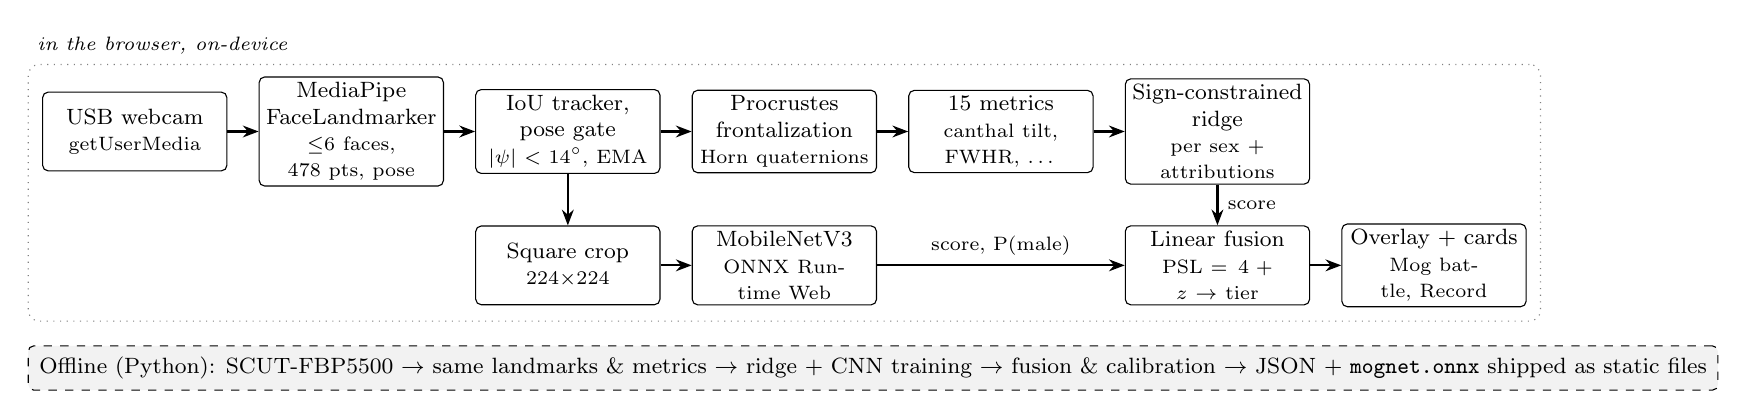
\begin{tikzpicture}[
  box/.style={draw, rounded corners=2pt, align=center, font=\footnotesize, minimum height=10mm,
              text width=22mm, inner sep=2pt, fill=white},
  arr/.style={-{Stealth[length=2mm]}, thick},
]
\node[box] (cam) at (0,0) {USB webcam\\\scriptsize getUserMedia};
\node[box] (mp)  at (2.75,0) {MediaPipe FaceLandmarker\\\scriptsize $\le$6 faces, 478 pts, pose};
\node[box] (trk) at (5.5,0) {IoU tracker, pose gate\\\scriptsize $|\psi|<14^\circ$, EMA};
\node[box] (fr)  at (8.25,0) {Procrustes frontalization\\\scriptsize Horn quaternions};
\node[box] (met) at (11,0) {15 metrics\\\scriptsize canthal tilt, FWHR, \dots};
\node[box] (geo) at (13.75,0) {Sign-constrained ridge\\\scriptsize per sex + attributions};
\node[box] (crop) at (5.5,-1.7) {Square crop\\\scriptsize $224{\times}224$};
\node[box] (cnn)  at (8.25,-1.7) {MobileNetV3\\\scriptsize ONNX Runtime Web};
\node[box] (fuse) at (13.75,-1.7) {Linear fusion\\\scriptsize PSL $=4+z$ $\rightarrow$ tier};
\node[box] (ui)   at (16.5,-1.7) {Overlay + cards\\\scriptsize Mog battle, Record};
\draw[arr] (cam) -- (mp); \draw[arr] (mp) -- (trk); \draw[arr] (trk) -- (fr);
\draw[arr] (fr) -- (met); \draw[arr] (met) -- (geo);
\draw[arr] (trk) -- (crop); \draw[arr] (crop) -- (cnn);
\draw[arr] (cnn) -- node[above, font=\scriptsize] {score, P(male)} (fuse);
\draw[arr] (geo) -- node[right, font=\scriptsize] {score} (fuse);
\draw[arr] (fuse) -- (ui);
\begin{scope}[on background layer]
  \node[draw=gray, dotted, rounded corners, fit=(cam)(geo)(crop)(ui), inner sep=5pt,
        label={[font=\scriptsize\itshape, anchor=south west]north west:in the browser, on-device}] (web) {};
\end{scope}
\node[draw, dashed, rounded corners=2pt, fill=gray!10, font=\footnotesize, inner sep=4pt, anchor=north west]
  at ([yshift=-3mm]web.south west) {Offline (Python): SCUT-FBP5500 $\rightarrow$ same landmarks \& metrics
  $\rightarrow$ ridge + CNN training $\rightarrow$ fusion \& calibration $\rightarrow$ JSON + \texttt{mognet.onnx}
  shipped as static files};
\end{tikzpicture}}
\caption{System architecture. The browser pipeline (top) and the offline training pipeline (bottom) share
the same landmark model, crop rule and metric code. The TypeScript metric implementation is checked
against the Python reference in unit tests.}
\Description{Block diagram of the pipeline.}
\label{fig:arch}
\end{figure*}

\subsection{Design process and ideation}
Our initial plan was a direct Omoggle-style design: a face mesh, looksmax ratios, and a score from
hand-picked ``ideal'' ranges for each ratio. Four findings during development reshaped it:
\begin{enumerate}[leftmargin=*,nosep]
  \item \textbf{Hand-picked ideals are arbitrary.} Their weights had no justification, and some community
        ideals do not match the measurements MediaPipe's landmarks produce. We switched to \emph{learning} the
        weights from 5,500 faces rated by 60 people~\cite{liang2018scut}.
  \item \textbf{Head pose leaks into every metric.} On the dataset, our symmetry metric correlated
        $r=0.97$ with $|\text{yaw}|$, so it was measuring head turn, not the face. Frontalization reduced
        this to $r=0.67$, and pose gating in the app handles the rest (\S\ref{sec:frontal}).
  \item \textbf{Unconstrained explanations contradict the data.} The metrics are correlated with each other
        (e.g.\ jaw\,:\,cheekbone width vs.\ jaw angle, $r=-0.75$; FWHR vs.\ face length\,:\,width, $r=-0.68$).
        An ordinary ridge regression therefore gave FWHR a large \emph{positive} weight (+0.26 for male and +0.46 for female
        faces, in rating units per SD), even though FWHR on its own correlates \emph{negatively} with
        ratings ($r\approx-0.25$). Users with a high FWHR would have been told it was a strength while the raw
        data says the opposite. We now constrain the signs (\S\ref{sec:geo}).
  \item \textbf{Camera pose $\neq$ apparent pose.} Our first pose gate used MediaPipe's transformation
        matrix. It rejected a frontal face near the edge of a multi-person frame, because the matrix includes
        the off-axis viewing angle. We now gate on the apparent pose from frontalization, which is what the
        metrics actually depend on.
\end{enumerate}
For the interface we chose a browser app over a native OpenCV window. A browser tab runs on any laptop
with any USB camera, can be shared as a link, and keeps everything on-device.
Live cards update five times per second, while the overlay is drawn on every frame.

\subsection{Landmarks, tracking and pose gating}
MediaPipe FaceLandmarker runs in \texttt{VIDEO} mode on the GPU delegate, falling back to CPU, with up to
six faces, and returns 478 normalized 3D landmarks per face. We read the \emph{apparent} head pose, yaw
$\psi$ and pitch, from the rotation that aligns the face to our frontal template (\S\ref{sec:frontal}). We do not use
MediaPipe's facial transformation matrix for this. That matrix measures rotation relative to the camera ray, so
in testing a perfectly frontal face near the edge of a wide frame read as $-17^\circ$ of yaw. The Procrustes
yaw correlates $r=0.99$ with MediaPipe's yaw on the centered dataset images, at about $1.2\times$ the scale. A greedy IoU tracker (match threshold 0.25, 1\,s
time-to-live) keeps a stable ID per person. Metrics are smoothed with an exponential moving average
($\alpha=0.15$) and updated \emph{only} while the face is near-frontal ($|\psi|<14^\circ$,
$|\text{pitch}|<20^\circ$). When someone turns away, the card says ``face the camera'' and the score is
frozen. This is a direct fix for the angle sensitivity reported for Omoggle.

\subsection{Frontalization}
\label{sec:frontal}
Landmarks are converted to pixel-space 3D ($x W, y H, z W$), centered, and scaled to unit RMS radius. We then
find the rotation that best aligns them to a mean frontal template using Horn's closed-form quaternion
method~\cite{horn1987closed}: the top eigenvector of a $4{\times}4$ symmetric matrix built from the
cross-covariance. The template is a generalized-Procrustes mean of 1,257 near-frontal \emph{training} faces.
Metrics are computed on the $x,y$ coordinates of the aligned shape, after removing residual roll so
that the line between the pupils is horizontal. The browser uses a Jacobi eigen-solver port of the same
algorithm. Unit tests check it against the Python reference within $10^{-3}$ on five faces, including
the most strongly turned faces in the dataset.

\subsection{The 15 metrics}
All lengths are normalized by the interpupillary distance (IPD) or the bizygomatic width, so the metrics do not depend
on how far someone is from the camera. Table~\ref{tab:metrics} gives the landmark definitions.

\begin{table}[t]
\caption{Metrics (MediaPipe landmark indices in parentheses).}
\label{tab:metrics}
\footnotesize
\begin{tabularx}{\linewidth}{@{}lX@{}}
\toprule
Metric & Definition \\
\midrule
Canthal tilt & mean angle of inner$\rightarrow$outer canthus vs.\ pupil line (133--33, 362--263); $+$ = outer higher \\
Eye spacing (ESR) & IPD (468--473) / bizygomatic width (234--454) \\
FWHR & bizygomatic width / height glabella--upper lip (9--0) \\
Midface ratio & pupil line--upper lip height / IPD \\
Lower third & (subnasale--menton) / (glabella--menton) (2, 152, 9) \\
Chin\,:\,philtrum & (lower lip--menton) / (subnasale--upper lip) (17--152, 2--0) \\
Nose\,:\,intercanthal & alar width (129--358) / intercanthal width (133--362) \\
Mouth\,:\,nose & mouth width (61--291) / alar width \\
Jaw\,:\,cheekbone & bigonial (172--397) / bizygomatic width \\
Lower\,:\,upper lip & lower-lip height (14--17) / upper-lip height (0--13) \\
Eye openness & mean lid aperture / eye width (159--145, 386--374) \\
Brow--eye distance & brow (105, 334) to upper lid, / IPD \\
Face length\,:\,width & forehead--menton (10--152) / bizygomatic width \\
Asymmetry & mean mirror error of 13 bilateral pairs about the midline, / IPD \\
Jaw angle & projected angle zygion--gonion--menton (234--172--152, 454--397--152) \\
\bottomrule
\end{tabularx}
\end{table}

\subsection{Explainable geometric model}
\label{sec:geo}
For each sex we standardize every metric ($z_i$, clipped to $\pm4$) and fit
\[
\hat y_{\text{geo}} = b + \sum_{i=1}^{15}\big(\beta_i z_i + \gamma_i (z_i^2-1)\big) + \text{pose terms},
\]
where the pose terms ($|\psi|$, $|\text{pitch}-\text{median}|$) absorb any remaining pose effects during training and are
set to zero at inference. In the \emph{sign-constrained} variant, $\operatorname{sign}(\beta_i)$ must match
the sign of metric $i$'s marginal correlation with the rating, and $\gamma_i\le0$, so any curvature can only
express an ``ideal range'' (an inverted U). We solve it as non-negative ridge regression on a re-signed
design matrix, with $\alpha$ chosen by 5-fold cross-validation. Because the model is additive, the contribution
$c_i=\beta_i z_i+\gamma_i(z_i^2-1)$ is exact and has zero mean over the training set, so it reads as
``points above or below an average face.'' The UI shows $c_i/\sigma_y$ in PSL units and the top three
positive and negative contributions. The ``top-tier average'' shown for each metric is that metric's mean
over the top 20\% of rated training faces of the same sex.

\subsection{CNN}
We fine-tune an ImageNet-pretrained MobileNetV3-Large~\cite{howard2019mobilenetv3} with a two-output
head (beauty score, sex logit; loss = smooth-L1 + $0.2\times$BCE). Crops are square boxes 1.35$\times$ the
landmark bounding box, black-padded, resized to $224{\times}224$. The browser uses exactly the same rule, so
training and live inputs are framed the same way. Training used 85\% of the official training split, with
15\% held out for validation. Settings: AdamW, one-cycle learning rate with a peak of $3{\times}10^{-4}$, batch 32,
25 epochs, flips, $\pm8^\circ$ affine and color jitter. We kept the epoch with the best validation correlation
($r=\bestValR$). The model is exported to ONNX (opset 17, 13.9\,MB) and runs in ONNX Runtime Web (WASM).
A round-robin scheduler sends one face to the CNN every 120\,ms, and the outputs are smoothed per track.

\subsection{Fusion and PSL calibration}
A linear regression on the validation set combines the two models:
$\hat y = \wCnn\,\hat y_{\text{cnn}} + \wGeo\,\hat y_{\text{geo}} + b$. We map to PSL with
$\text{PSL}=4+(\hat y-\mu)/\sigma$, where $\mu=\scoreMean$ and $\sigma=\scoreStd$ are the mean and SD of the
human ratings, clipped to $[1,8]$. With this mapping the community tier cut-offs land on familiar percentiles: MTN
covers the middle (3.75--4.5), HTN is roughly the top 31\%, Chadlite the top 10\% ($\ge5.25$), and Chad the top
2.3\% ($\ge6$). The detected sex chooses the geometric model and the tier names, and users can correct it by
clicking the sex badge on their card.

\subsection{Interface and privacy}
The app is built with React and TypeScript on Vite. Everything is drawn on one canvas: the video, corner-bracket boxes
colored by tier, the PSL and tier label, and optional guides and mesh. All model files and wasm runtimes are
served from the app itself, so it also works offline on demo day. No frame is ever sent over the network;
Snapshot and Record save files locally. Record logs \emph{numbers only} (per-person PSL, model
outputs, yaw, fps). An opening screen asks for confirmation that everyone in frame is 18+ and has consented.

\subsection{Replicating the system}
All code is in our repository. \texttt{README.md} lists the nine commands that rebuild every model and
number in this paper from the public dataset, and \texttt{npm run dev} starts the app. Every number in this
document is generated from the result files by \texttt{make\_figures.py}.

% ---------------------------------------------------------------------------------------------------
\section{Evaluation}

\subsection{Agreement with human raters}

\begin{table}[t]
\caption{SCUT-FBP5500 official 60/40 split (test $n=\nTest$). Target: mean rating of 60 raters (1--5).}
\label{tab:results}
\footnotesize
\begin{tabular}{@{}lccc@{}}
\toprule
Model & Pearson $r$ $\uparrow$ & MAE $\downarrow$ & RMSE $\downarrow$ \\
\midrule
AlexNet~\cite{liang2018scut} & 0.8298 & -- & -- \\
ResNet-18~\cite{liang2018scut} & 0.8513 & -- & -- \\
ResNeXt-50~\cite{liang2018scut} & 0.8777 & -- & -- \\
\midrule
Ours: geometry only (constrained ridge) & \geoR & \geoMAE & \geoRMSE \\
Ours: MobileNetV3 CNN & \cnnR & \cnnMAE & \cnnRMSE \\
Ours: fused (deployed) & \textbf{\fusedR} & \textbf{\fusedMAE} & \textbf{\fusedRMSE} \\
\bottomrule
\end{tabular}
\end{table}

Table~\ref{tab:results} and Figure~\ref{fig:scatter} show the results. The fused model reaches $r=\fusedR$
on the held-out test split. That is higher than all three of the dataset paper's 60/40 baselines, although
it is below recent large research models ($\approx$0.92~\cite{boukhari2025synergynet}), which are not
designed for real-time use in a browser. The geometry-only model ($r=\geoR$) is much weaker than the CNN. Proportions explain a large part
of attractiveness, but skin, hair, expression and other texture cues matter too. Its value is in
the explanations. The sex head reaches \sexAcc\% accuracy. On the PSL scale the mean absolute error is
\pslMAE\ points, the exact tier matches in \tierExact\% of test faces, and the tier is within one step in
\tierWithinOne\%.

\begin{figure}[t]
\centering
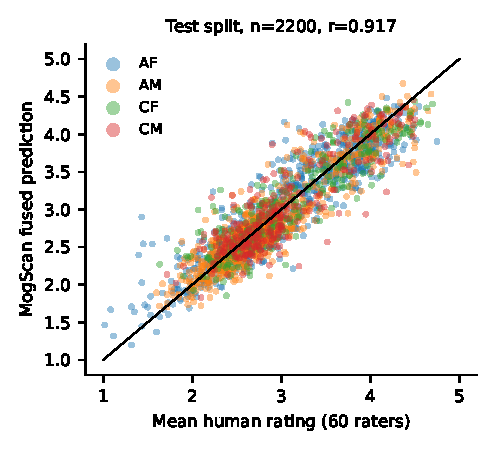
\includegraphics[width=0.9\linewidth]{figures/scatter.pdf}
\caption{Fused prediction vs.\ mean human rating on the test split, colored by subgroup (A/C = Asian/Caucasian, F/M).}
\Description{Scatter plot.}
\label{fig:scatter}
\end{figure}

\subsection{Do looksmax rules hold up?}
Figure~\ref{fig:metric_corr} shows each metric's raw correlation with the human rating, measured on
frontalized landmarks. The strongest single metric is \emph{\topMetric} ($r=\topMetricR$, averaged
across sexes). Several community rules do \emph{not} hold up for these raters:
\begin{itemize}[leftmargin=*,nosep]
  \item \textbf{Canthal tilt}, the best-known looksmax metric, has essentially no correlation ($r\approx0.00$). Before
        frontalization it seemed to matter ($r\approx0.28$), but that came from head pose.
  \item \textbf{``Hunter eyes'':} more \emph{open} eyes go with higher ratings ($r\approx0.37$).
  \item \textbf{Wide jaw and high FWHR:} faces that are \emph{narrower} in the jaw relative to the cheekbones
        ($r\approx-0.38$), with lower FWHR ($r\approx-0.26$) and softer projected jaw angles ($r\approx0.36$), are rated higher.
        That is a V-shaped face, the opposite of the ``wide, square jaw'' ideal.
  \item \textbf{Symmetry} looks \emph{negatively} related to attractiveness on the full dataset, but the effect disappears
        ($r\approx0.00$) for faces within $3^\circ$ of frontal. It comes from residual pose, since head-turned photos received higher
        ratings ($r=0.28$ for $|\text{yaw}|$, male faces).
\end{itemize}
A longer chin relative to the philtrum ($r\approx0.19$) and wider-set eyes ($r\approx0.19$) agree with
community advice. These results describe one dataset and one rater panel, and East Asian beauty norms may favour
V-shaped faces. Still, they show why MogScan displays the \emph{data-derived} target next to the community range
instead of repeating forum rules, and why pose control is necessary for any measurement-based rating.

\begin{figure}[t]
\centering
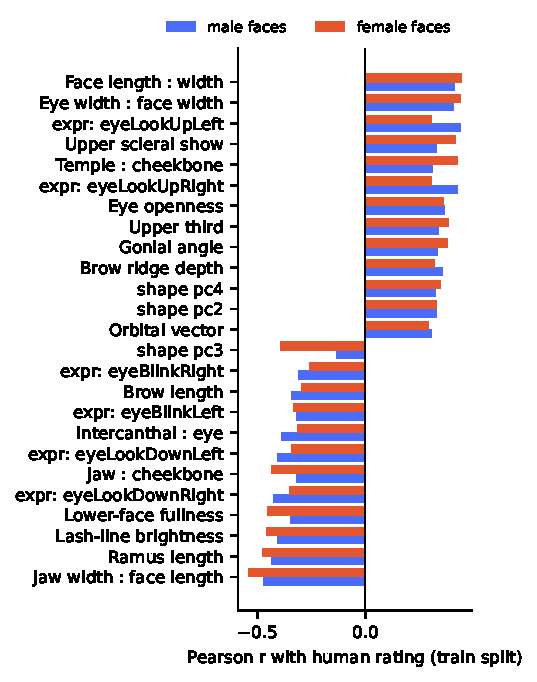
\includegraphics[width=0.95\linewidth]{figures/metric_corr.pdf}
\caption{Correlation of each frontalized metric with human ratings (training split), split by sex.}
\Description{Horizontal bar chart of correlations.}
\label{fig:metric_corr}
\end{figure}

\subsection{Subgroup bias}

\begin{table}[t]
\caption{Fused model by subgroup (test split). Signed bias = mean(pred $-$ human).}
\label{tab:bias}
\footnotesize
\begin{tabular}{@{}lcccc@{}}
\toprule
Group & $n$ & $r$ & MAE & Signed bias \\
\midrule
\csname @@input\endcsname generated/bias_table.tex
\bottomrule
\end{tabular}
\end{table}

Table~\ref{tab:bias} breaks the error down by the dataset's four subgroups. SCUT-FBP5500 has only Asian and
Caucasian faces, rated by one panel of 60 young raters. \textbf{People of other ethnicities are not
represented at all}, so the model's behaviour on them is unvalidated. That is a serious limitation for
a consumer product. The app's opening screen says so, and collecting a more diverse dataset is our first
item of future work.

\subsection{User study}
\label{sec:study}
\ifdefined\studyPending
\pending{The user study has not been run yet. Follow study/protocol.md with 8--15 participants, export the
Google Form to study/responses.csv and the session logs to study/logs/, run analyze\_survey.py,
analyze\_logs.py and make\_figures.py, then rebuild this PDF. Every number in this section is filled in
automatically. Do not type numbers by hand.}
\else
We ran \studyN\ adult participants in groups of 2--3 (protocol in \texttt{study/protocol.md}). Each
person did a solo scan, then a group scan with Mog battle on, then a survey. Usability was \textbf{SUS
\susMean} ($SD=\susSD$)~\cite{brooke1996sus}, and the Net Promoter Score~\cite{reichheld2003one} was \textbf{\npsScore}.
\agreeAcc\% agreed that the score felt accurate, \agreeFeatures\% that the feature list was useful,
\agreeGroup\% that group scanning was fun, and \agreePrivacy\% that on-device processing made them more
comfortable. \payPct\% would pay for an extended version. As a wellbeing check, \agreeFeelbad\% agreed that
MogScan made them feel worse about their appearance (Figure~\ref{fig:likert}).
\begin{figure}[t]
\centering
\includegraphics[width=\linewidth]{figures/survey_likert.pdf}
\caption{Survey responses (5-point Likert).}
\Description{Diverging stacked bar chart of Likert responses.}
\label{fig:likert}
\end{figure}
\fi

\subsection{Performance and stability}
\ifdefined\logsPending
\pending{Fill from study logs (median PSL std.\ while still, median fps).} In our own development testing (Chrome on an Apple-silicon MacBook,
photo mode, one face) the full pipeline ran at about 27--36 frames per second.
\else
Across \logSessions\ recorded sessions (\logTracks\ person-tracks), the median frame rate was
\fpsMedian\,fps, and the median standard deviation of a person's PSL over a track was \pslStd\ points.
\fi

% ---------------------------------------------------------------------------------------------------
\section{Ethics, Risks and Limitations}
\label{sec:ethics}
Rating faces can hurt people. Parental-safety reviewers rate PSL apps 18+ and warn that they can reinforce
body dissatisfaction~\cite{bark2026psl}. Our mitigations:
\begin{itemize}[leftmargin=*,nosep]
  \item an 18+ and consent screen;
  \item on-device processing with no storage;
  \item ``Kind'' wording by default;
  \item honest framing in the app (``a model's estimate of how one panel judged faces, not your worth'');
  \item a wellbeing item in our survey.
\end{itemize}
Technical limitations:
\begin{itemize}[leftmargin=*,nosep]
  \item SCUT faces are studio-like frontal photos, while webcam frames vary in lighting and lens distortion, so there is
        domain shift;
  \item the mesh starts at the upper forehead, so true facial thirds and full face length are approximations;
  \item the jaw angle is a 2D projection;
  \item the dataset covers two ethnic groups and only binary sex labels.
\end{itemize}
Commercial use would require licensed training data.

\section{Future Work}
\begin{itemize}[leftmargin=*,nosep]
  \item \textbf{Diverse, licensed data:} collect consented ratings across many ethnicities, ages and rater groups, retrain,
        and publish subgroup error before any commercial launch.
  \item \textbf{Side-profile scan:} gonial angle, chin projection and the Ricketts E-line need a profile view. Prompt users to turn
        their head and fuse the measurements.
  \item \textbf{Streamer overlay:} an OBS browser source with a transparent background and battle ELO, aimed at
        the creators who popularized Omoggle.
  \item \textbf{Progress tracking and glow-up plan:} longitudinal, pose-normalized measurements with evidence-based,
        non-surgical suggestions (grooming, skin care, posture). Never surgery prompts.
  \item \textbf{Better CNN explanations:} Grad-CAM heatmaps for the texture cues the geometric model cannot see, and a WebGPU
        backend for higher frame rates with six people in frame.
\end{itemize}

\bibliographystyle{ACM-Reference-Format}
\bibliography{references}

\end{document}
